\subsection{Automation}
\label{sec:automation}

\textbf{Purpose}: Performing growth-, maintenance-, and data-related tasks autonomously on the basis of both schedule and necessity to reduce crew maintenance time, improve consistency of products, and eliminate safety risks. Maintains the homogeneity of the internal environment with increased accuracy and precision over crew interference, while enabling simultaneous control over all parameters.

\textbf{Function}:
\begin{itemize}
    \item \textbf{Inputs}: Environment data stream (sensor readings), growth program
    \item \textbf{Outputs}: Actuator control signals, crew/cloud messaging, environment data (stored), timelapse photo set
\end{itemize}

\textbf{Method}:
\begin{enumerate}
    \item \textit{Setup}:
    \begin{enumerate}
        \item Power is connected and system is booted;
        \item Program is selected by user;
    \end{enumerate}
    \item \textit{Testing}:
    \begin{itemize}
        \item Power-on Self-Test (POST) passes (i.e. all hardware is online and communicating as expected).
        \item Systems enact program as intended (i.e. control systems respond properly).
    \end{itemize}
    \item \textit{Process}:
    \begin{enumerate}
        \item Checks operating preconditions (self POST and per-subsystem);
        \item \textbf{Environment Control Loop} (matches \textit{Sense-Plan-Act} model of robotics): %TODO cite the model
        \begin{enumerate}
            \item \textit{Sense}: Receives and stores data about current environment state;
            \item \textit{Plan}: Compares current state to "desired"/program state, develops a "plan"/actuator control to reach desired state;
            \item \textit{Act}: Controls subsystem operations in order to enact the plan;
        \end{enumerate}
        \item Notifies user on maintenance requirement (i.e. non-automated input/output management, refills, repairs, etc.), end-of-program (EoP), and diagnostic info;
    \end{enumerate}
    \item \textit{Shutdown} (either manual or EoP):
    \begin{enumerate}
        \item Stop all subsystem operations;
        \item Power down;
    \end{enumerate}
\end{enumerate}

\clearpage

\textbf{Features}:

A dual-computer system was chosen to allow for discrete management of high-level functionality (camera capture, internet/cloud functionality, local storage, complex calculations, etc.) and low-level functionality (hardware-level communications, actuator control and GPIO) in a master/slave topology with a constant two-way stream of shared data.

\begin{itemize}
    \item \textit{Computer (Master)} \cite{raspberrypi}: Manages data collection, batch storage, analysis, and transmission/receiving, as well as planning/calculations for actuator control. Includes internal clock (for program, notification), network connection (for data transmission, notification), photo capture, and non-volatile storage (for data/photos). Sends instructions derived from the program to the microcontroller.
    \item \textit{Microcontroller (Slave)} \cite{arduino}: Manages detailed sensor/actuator states and communications (on/off, sensor readings, actuator control). Streams collected sensor readings to the computer.
    \item \textit{Program}: Set of actuated instructions (e.g. lights on) and control targets (e.g. hold air temperature at 22°C) to enact at specific points in the growth cycle, as well as config data;
    \item \textit{Camera Capture \& Plant Performance Metric (PPM) Extraction}: Top-down and side-view cameras \cite{camera}, captured under standard lighting at regular intervals throughout the course of the growth cycle. For live feed transmission to users (local and remote), as well as PPM extraction via computer vision and machine learning for yield and diagnostic analysis. Potentially relevant PPMs include (but are not limited to):
    \begin{itemize}
        \item Leaf health indicators (i.e. leaf tip burn, leaf curl, chlorosis);
        \item Leaf count, size distribution;
        \item Leaf density;
        \item Canopy dimensions/surface area;
        \item Plant height;
        \item Fruit/harvest body size, ripeness;
    \end{itemize}
    \item \textit{Environment Data}: Record the environment's current state. Covers each \textit{control system} environment parameter (e.g. included in a feedback loop). Control system environment parameters include:
    \begin{itemize}
        \item Leaf-zone temperature (see \ref{sec:airthermoregulation});
        \item Leaf-zone humidity (see \ref{sec:humidityregulation});
        \item Root-zone temperature (see \ref{sec:aeroponics});
        \item Gas concentrations (see \ref{sec:gas});
    \end{itemize}
    \item \textit{Actuator Control}: Induces change in environment parameters. Covers both \textit{control system} and \textit{actuated instruction} environment parameters. Actuated instruction environment parameters include:
    \begin{itemize}
        \item Lighting (see \ref{sec:lighting});
        \item Water delivery (see \ref{sec:aeroponics});
        \item Plant nutrient delivery (see \ref{sec:aeroponics});
        \item Water pH (see \ref{sec:aeroponics});
        \item Air circulation rate (see \ref{sec:airthermoregulation});
    \end{itemize}
    \item \textit{Diagnostic Systems}: Include informative sensors tracking system input availability, subsystem diagnostics, etc. as well as notification triggers.
\end{itemize}

\clearpage

\textbf{Figures}

\begin{figure}[h!]
    \centering
    \frame{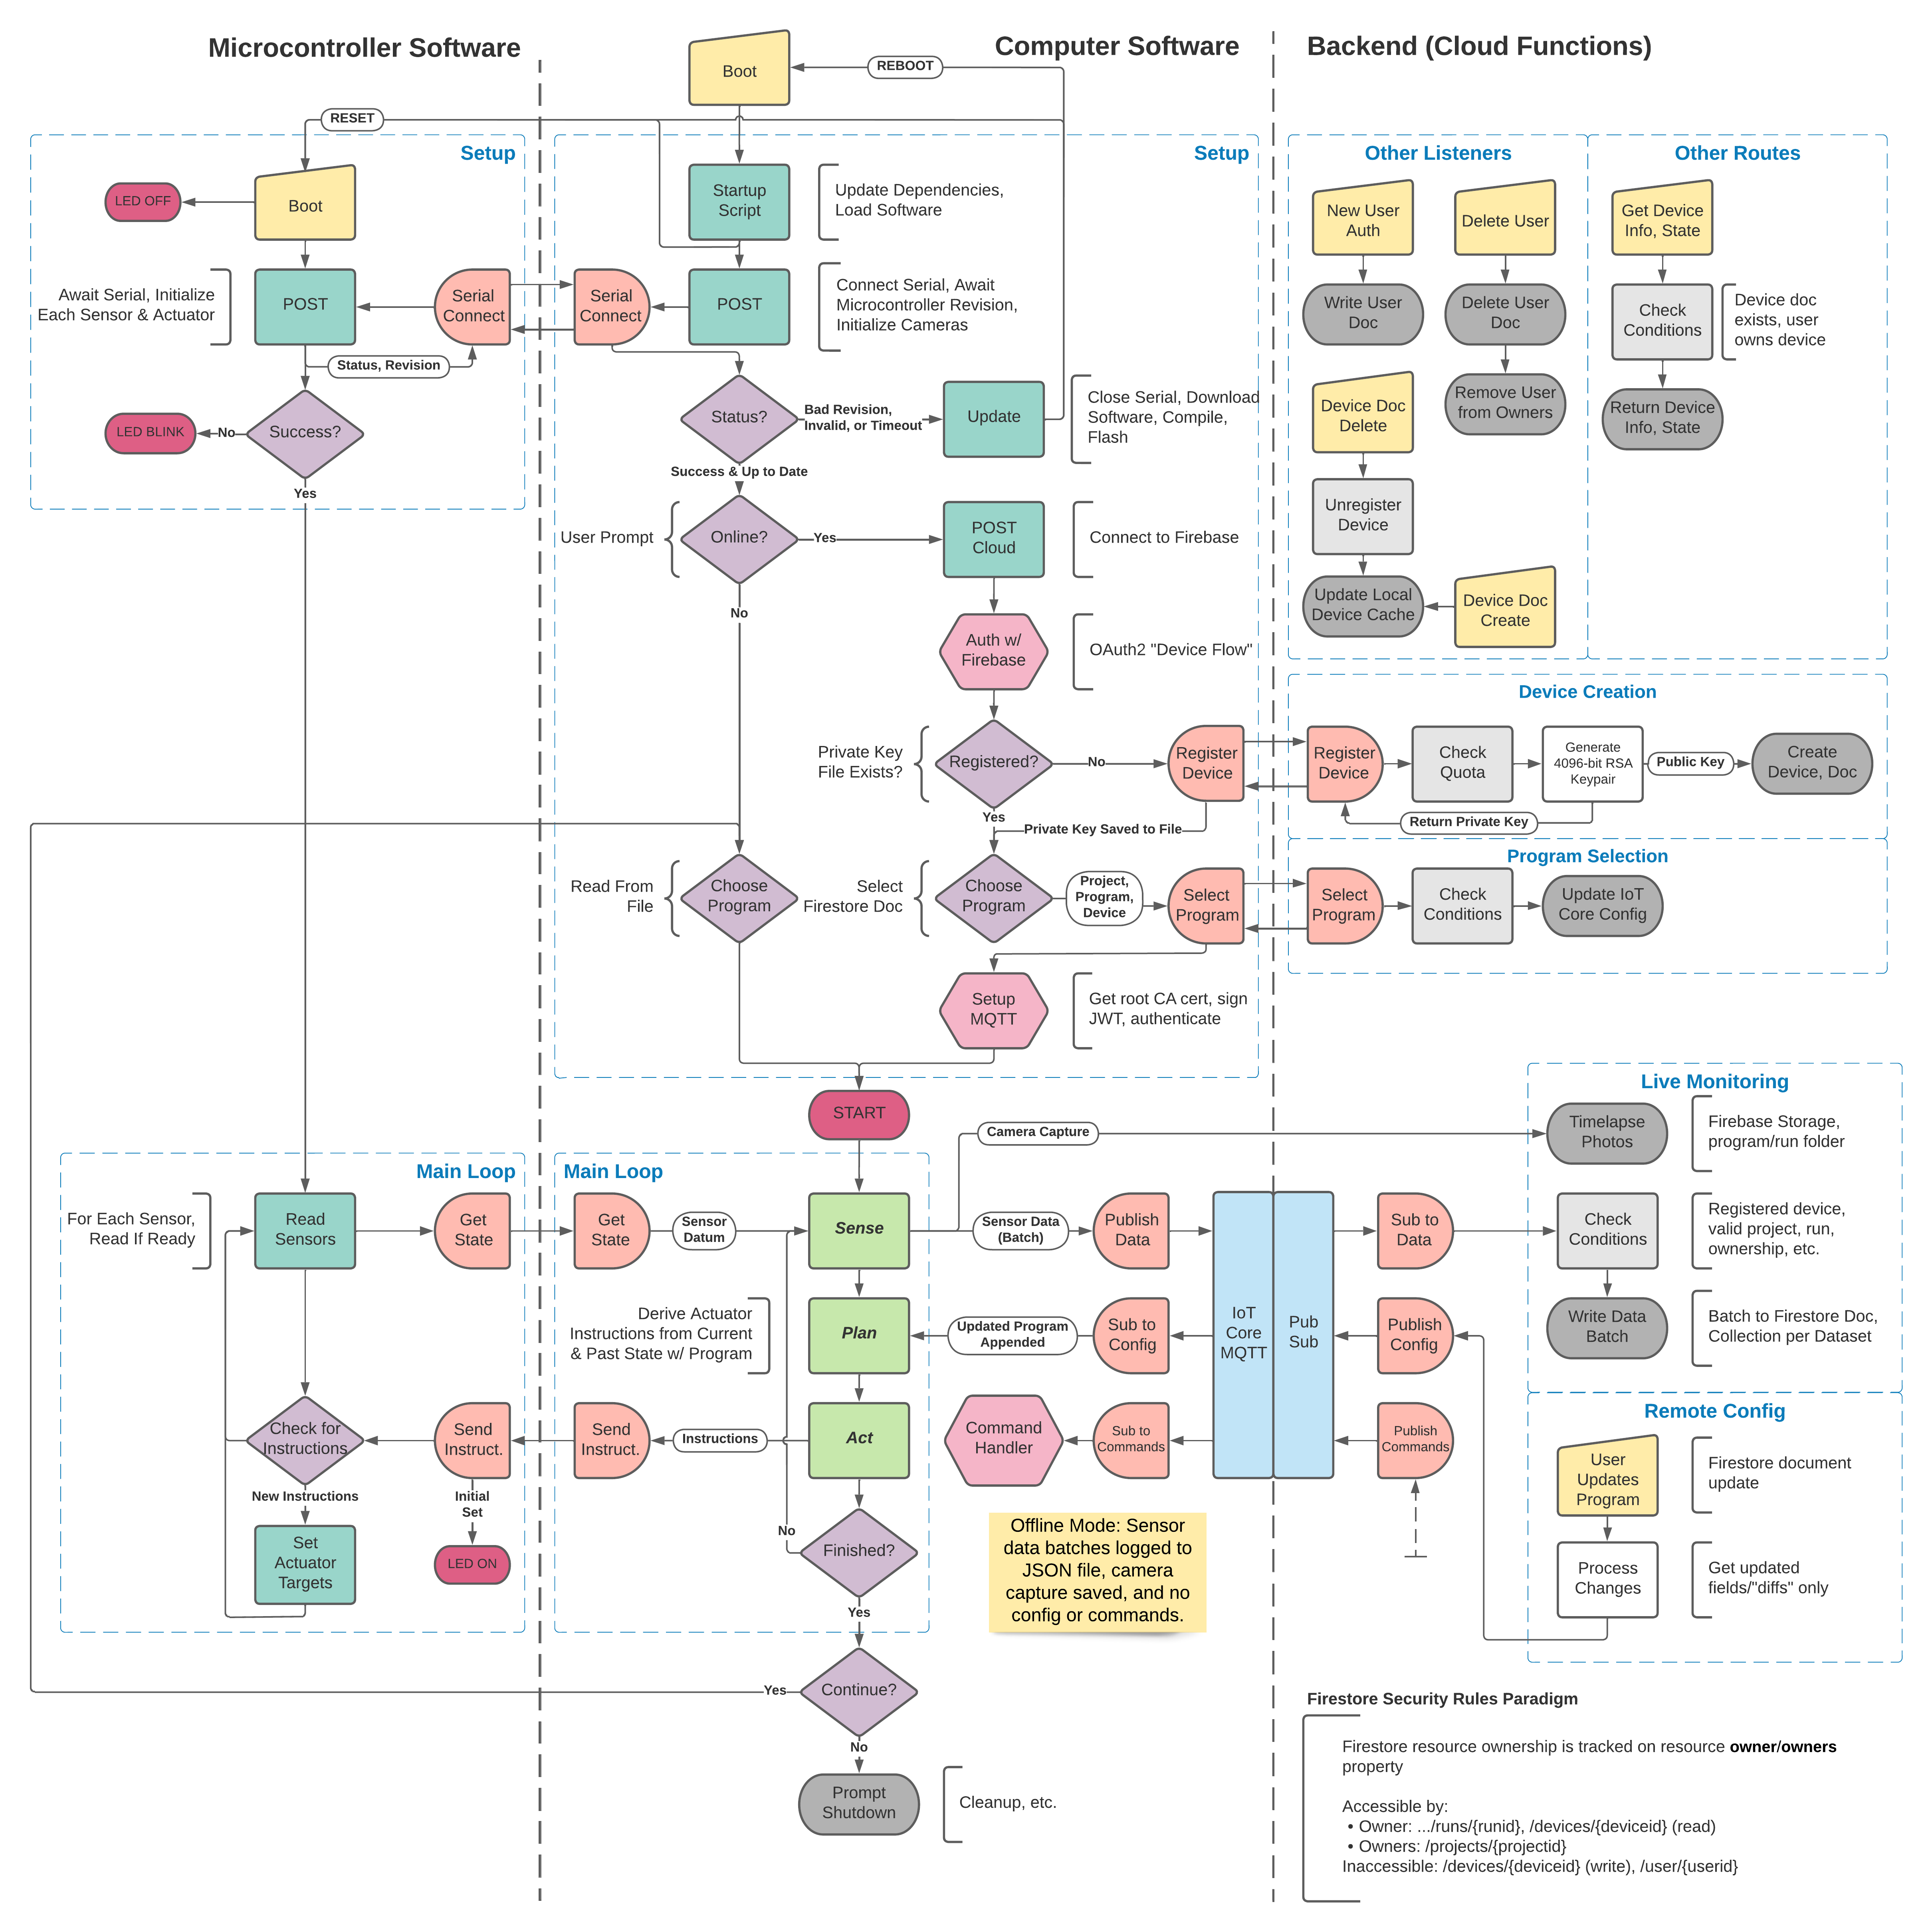
\includegraphics[width=\textwidth]{../assets/figures/automation_software.png}}
    \caption{Software control flow diagram.}
    \label{fig:automation_software}
\end{figure}

\begin{figure}[h!]
    \centering
    \frame{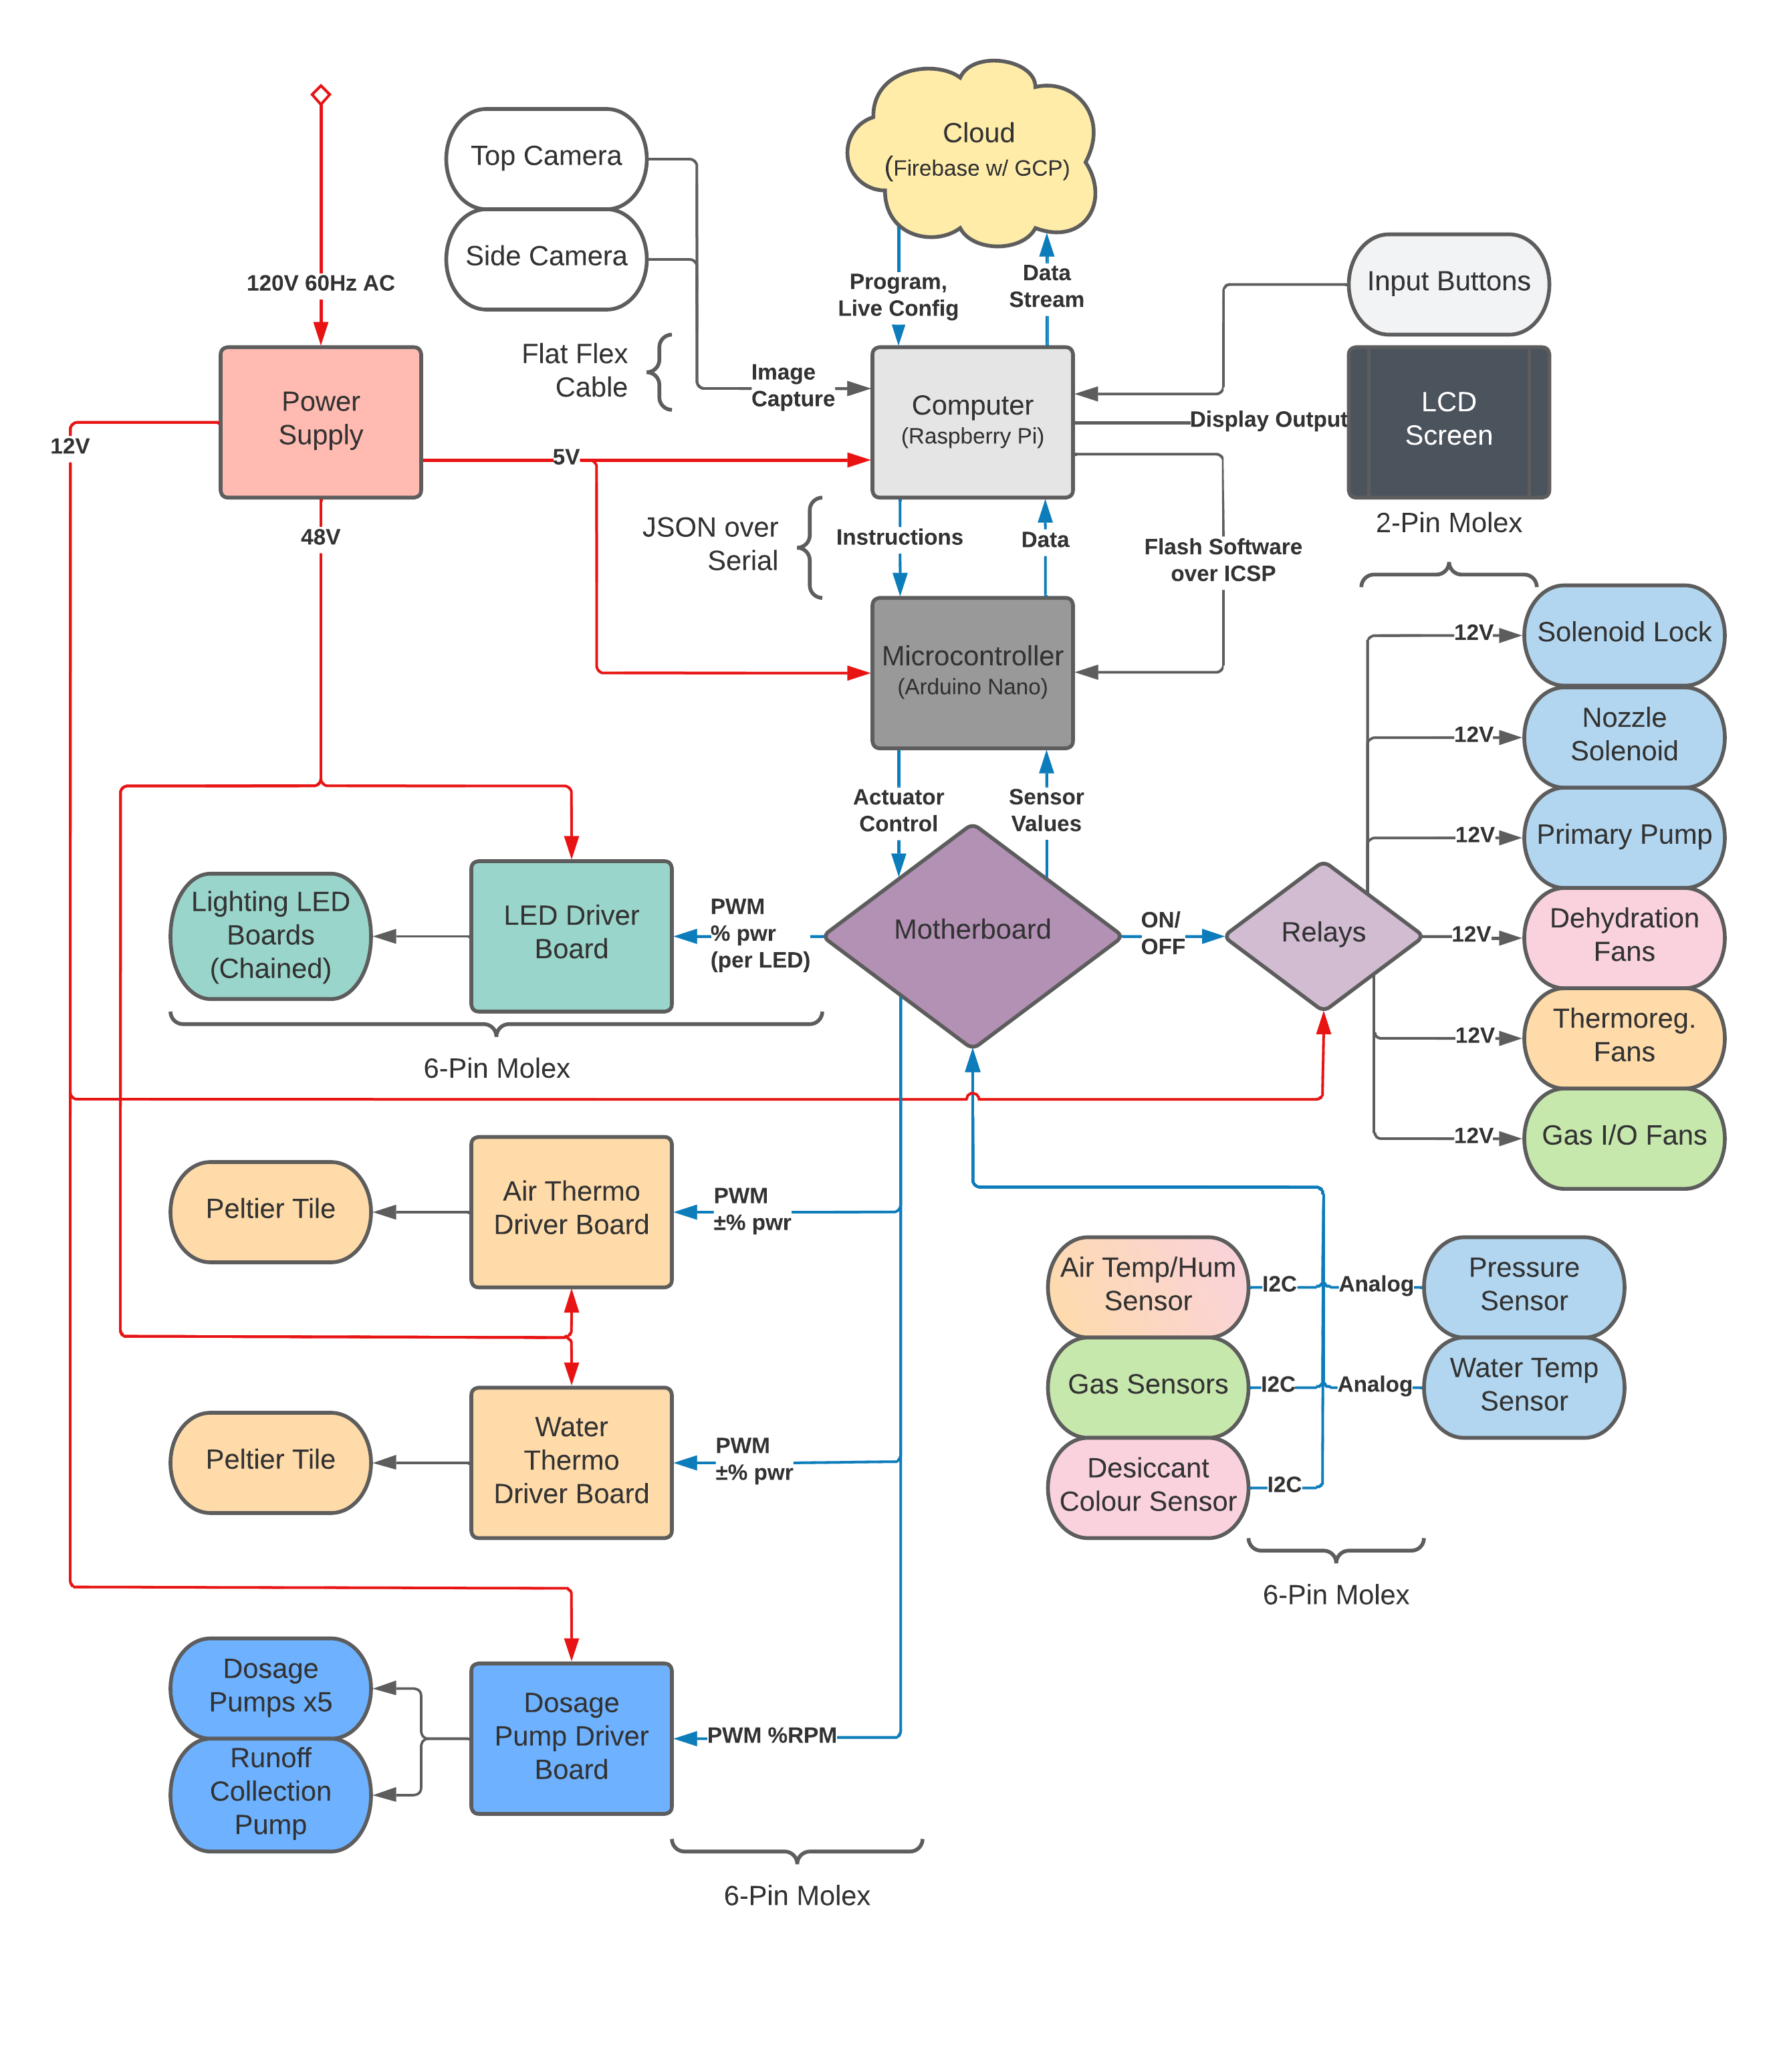
\includegraphics[width=\textwidth]{../assets/figures/automation_wiring.png}}
    \caption{System wiring diagram.}
    \label{fig:automation_wiring}
\end{figure}